\documentclass{article}
\usepackage{tikz}
\usepackage{amsmath}

\begin{document}

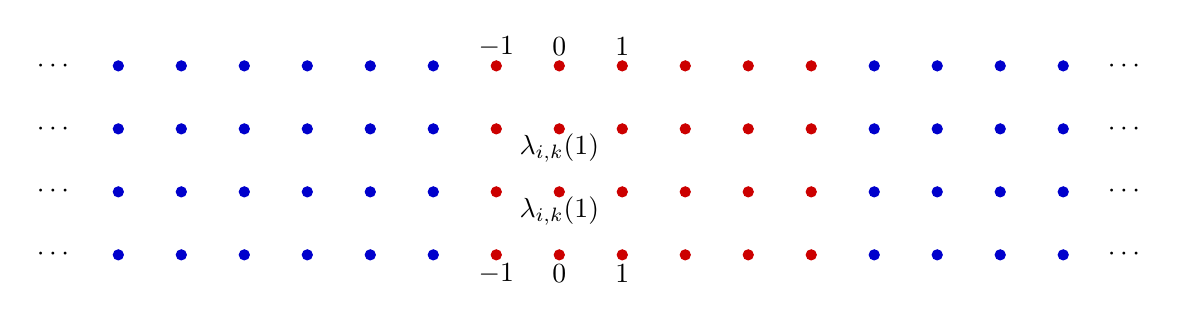
\begin{tikzpicture}[scale=0.8]
    % Define colors
    \colorlet{bluecolor}{blue!80!black}
    \colorlet{redcolor}{red!80!black}
    
    % Draw horizontal lines with dots
    \foreach \y in {0, 1, 2, 3} {
        % Blue dots (left side)
        \foreach \x in {-7, -6, -5, -4, -3, -2} {
            \filldraw[bluecolor] (\x, -\y) circle (0.08);
        }
        
        % Red dots (middle)
        \foreach \x in {-1, 0, 1, 2, 3, 4} {
            \filldraw[redcolor] (\x, -\y) circle (0.08);
        }
        
        % Blue dots (right side)
        \foreach \x in {5, 6, 7, 8} {
            \filldraw[bluecolor] (\x, -\y) circle (0.08);
        }
        
        % Ellipsis on both sides
        \node at (-8, -\y) {$\cdots$};
        \node at (9, -\y) {$\cdots$};
    }
    
    % Labels for first row
    \node at (-1, 0.3) {$-1$};
    \node at (0, 0.3) {$0$};
    \node at (1, 0.3) {$1$};
    
    % Labels for second row
    \node at (0, -1.3) {$\lambda_{i,k}(1)$};
    
    % Labels for third row
    \node at (0, -2.3) {$\lambda_{i,k}(1)$};
    
    % Labels for fourth row
    \node at (-1, -3.3) {$-1$};
    \node at (0, -3.3) {$0$};
    \node at (1, -3.3) {$1$};
\end{tikzpicture}

\end{document}